%%%%%%%%%%%%%%%%%%%%%%%%%%%%%%%%%%%%%%%%%%%%%%%%%%%%%%%%%%
\frame {\frametitle{Spark's Storage Module}
%%%%%%%%%%%%%%%%%%%%%%%%%%%%%%%%%%%%%%%%%%%%%%%%%%%%%%%%%%
\begin{itemize}
	\item {\bf The storage module}
	\begin{itemize}
		\item Access (I/O) ``external'' data sources: HDFS, Local Disk, RAM, remote data access through the network
		\item Caches RDDs using a variety of ``storage levels''
	\end{itemize}

	\vspace{20pt}

	\item {\bf Main components}
	\begin{itemize}
		\item The Cache Manager: uses the Block Manager to perform caching
		\item The Block Manager: distributed key/value store
	\end{itemize}
\end{itemize}
}

%%%%%%%%%%%%%%%%%%%%%%%%%%%%%%%%%%%%%%%%%%%%%%%%%%%%%%%%%%
\frame {\frametitle{Class Diagram of the Caching Component}
%%%%%%%%%%%%%%%%%%%%%%%%%%%%%%%%%%%%%%%%%%%%%%%%%%%%%%%%%%
\begin{figure}[h]
	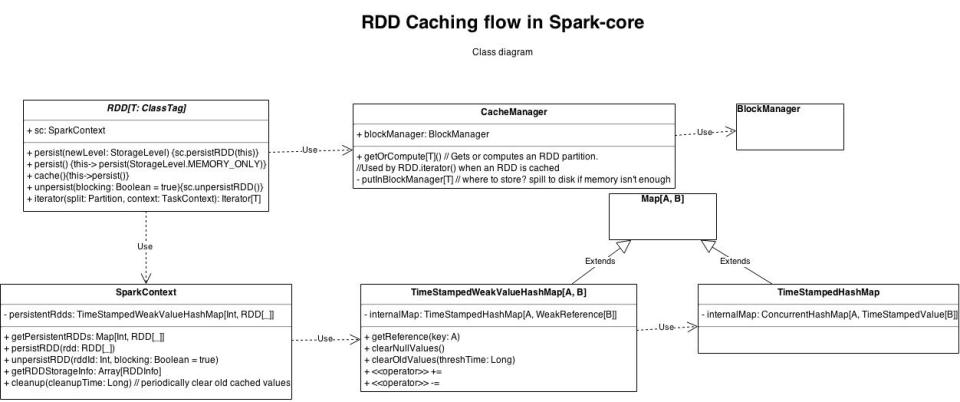
\includegraphics[scale=0.35]{./Figures/cache_classes}
\end{figure}
}

%%%%%%%%%%%%%%%%%%%%%%%%%%%%%%%%%%%%%%%%%%%%%%%%%%%%%%%%%%
\frame {\frametitle{How Caching Works}
%%%%%%%%%%%%%%%%%%%%%%%%%%%%%%%%%%%%%%%%%%%%%%%%%%%%%%%%%%
\begin{itemize}
	\item {\bf Frequently used RDD can be stored in memory}
	\begin{itemize}
		\item Deciding which RDD to cache is an art!
		\item One method, one short-cut: \texttt{persist()}, \texttt{cache()}
	\end{itemize}

	\vspace{20pt}

	\item {\bf \texttt{SparkContext} keeps track of cached RDD}
	\begin{itemize}
		\item Uses a data-structed called \texttt{persistentRDD}
		\item Maintains references to cached RDD, and eventually call the garbage collector
		\item Time-stamp based invalidation using \texttt{TimeStampedWeakValueHashMap[A, B]}
	\end{itemize}
\end{itemize}
}

%%%%%%%%%%%%%%%%%%%%%%%%%%%%%%%%%%%%%%%%%%%%%%%%%%%%%%%%%%
\frame {\frametitle{How Caching Works}
%%%%%%%%%%%%%%%%%%%%%%%%%%%%%%%%%%%%%%%%%%%%%%%%%%%%%%%%%%
\begin{columns}[t, onlytextwidth]
	\column[T]{.3\textwidth}
		
			\begin{figure}[h]
			  \centering
			  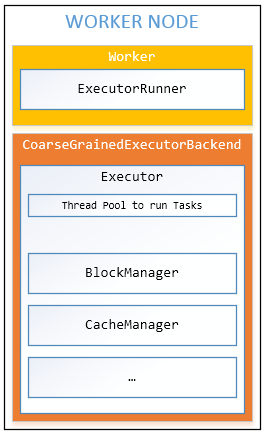
\includegraphics[scale=0.45]{./Figures/cache_workers}
			  \label{fig:spark_caching_workers}
			\end{figure}
	
	\column[T]{.6\textwidth}
		
			\begin{figure}[h]
			  \centering
			  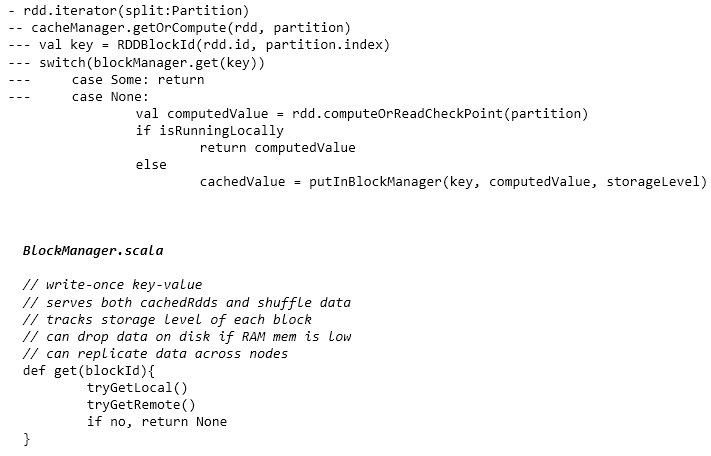
\includegraphics[scale=0.4]{./Figures/cache_stack}
			  \label{fig:caching_stack_calls}
			\end{figure}

\end{columns}
}

%%%%%%%%%%%%%%%%%%%%%%%%%%%%%%%%%%%%%%%%%%%%%%%%%%%%%%%%%%
\frame {\frametitle{The Block Manager}
%%%%%%%%%%%%%%%%%%%%%%%%%%%%%%%%%%%%%%%%%%%%%%%%%%%%%%%%%%
\begin{itemize}
	\item {\bf ``Write-once'' key-value store}
	\begin{itemize}
		\item One node per worker
		\item No updates, data is immutable
	\end{itemize}

	\vspace{20pt}

	\item {\bf Main tasks}
	\begin{itemize}
		\item Serves shuffle data (local or remote connections) and cached RDDs
		\item Tracks the ``Storage Level'' (RAM, disk) for each block
		\item Spills data to disk if memory is insufficient
		\item Handles data replication, if required
	\end{itemize}
\end{itemize}
}

%%%%%%%%%%%%%%%%%%%%%%%%%%%%%%%%%%%%%%%%%%%%%%%%%%%%%%%%%%
\frame {\frametitle{Storage Levels}
%%%%%%%%%%%%%%%%%%%%%%%%%%%%%%%%%%%%%%%%%%%%%%%%%%%%%%%%%%
\begin{itemize}
	\item {\bf The Block Manager can hold data in various storage tiers}
	\begin{itemize}
		\item \texttt{org.apache.spark.storage.StorageLevel} contains flags to indicate which tier to use
		\item Manual configuration, in the application
		\item Deciding the storage level to use for RDDs is not trivial
	\end{itemize}

	\vspace{10pt}

	\item {\bf Available storage tiers}
	\begin{itemize}
		\item RAM (default option): if the the RDD doesn't fit in memory, some partitions will not be cached (will be re-computed when needed)
		\item Tachyon (off java heap): reduces garbage collection overhead, the crash of an executor no longer leads to cached data loss
		\item Disk
	\end{itemize}

	\vspace{10pt}

	\item {\bf Data format}
	\begin{itemize}
		\item Serialized or as Java objects
		\item Replicated partitions
	\end{itemize}
\end{itemize}
}
